\documentclass{report}
\usepackage{fullpage}
\usepackage{amssymb}
\setcounter{tocdepth}{4}
\usepackage[pdftex]{graphicx}
\usepackage{thumbpdf}

\usepackage{url}

\urldef{\mailsa}\path|{h.cunningham, k.bontcheva, v.tablan, i.roberts,
m.agatonovic, d.damljanovic, n.aswani, t.heitz}@dcs.shef.ac.uk|
\newcommand{\keywords}[1]{\par\addvspace\baselineskip\noindent\keywordname\enspace\ignorespaces#1}
\newcommand{\thing}{GATE Teamware User Guide}
\usepackage[
  pdftex,
  pdfborder=0,                %comment to get boxes around links
  pdftitle={GATE Teamware User Guide},
  pdfauthor={GATE Team},
  pdfsubject={GATE Teamware User Guide},
  pdfkeywords={},
  pdfpagemode=None,
  bookmarksopen=true
]{hyperref}

% first the title is needed
\title{GATE Teamware User Guide}

% a short form should be given in case it is too long for the running head

\author{GATE Team}
%

% (feature abused for this document to repeat the title also on left hand pages)

% the affiliations are given next

\begin{document}

\maketitle{}

\tableofcontents

\chapter{Introduction}
GATE Teamware  is a software suite and a methodology for the implementation and
support of \emph{annotation factories}: it is intended to provide a framework
for commercial annotation services, supplied either as in-house units or as
outsourced specialist activities. This framework is a novel development in
several aspects:
\begin{itemize}
  \item it structures intervention by different actors (human and machine)
  into clearly-defined roles and provides the means to manage them in a
  unified fashion,
  \item it complements GATE's developer-oriented facilities with User
  Interfaces (UIs) oriented on other necessary staff roles,
  \item it is methodological instead of purely technological.
\end{itemize}

\section{Roles}
There are a number of staff roles required for an effective annotation factory
including:
\begin{itemize}
  \item \textbf{annotators}, who are largely unskilled, may be
  geographically distributed, and whose work is quality controlled by curators
  via metrics-related mechanisms,
  \item \textbf{curators}, who may be skilled annotators, capable of making
  decisions and valuing annotator's work,
  \item \textbf{language engineers}, these staff work on resources producing
  automatic annotations. These resources are combined to produce a service.
  \item \textbf{managers}, who are supposed to create and manage annotation
  projects
  \item \textbf{administrators}, who administrate the workflow system and its
  users.
  \item \textbf{superadministrator}, single super user who can modify the
  critical parts of the application along with other administrator
  duties 
\end{itemize}
GATE Teamware, together with GATE Developer, provides tools for all these roles,
and the workflow by which they may be combined with automatic Information Extraction
(IE) systems to provide cost-effective annotation services.

\section{Prerequisites}
GATE Teamware is a Java web application deployable under Apache Tomcat server
(5.5.x and 6.x) and fully compatible with both JDK 1.5 and 1.6. 
Apart from a web browser (the currently supported versions are Internet
Explorer (versions: 6, 7 and 8), Firefox 1.5, 2.x, 3.x) and Opera (versions: 8,
9 and 10)) you need to have Java Web Start (JWS) version 1.6.0 installed on
client machines. JWS can be downloaded as the part of Java Runtime Environment
(JRE) version 6 from the following address:
\url{http://java.sun.com/javase/downloads/index.jsp}

\section{Login}
GATE Teamware authentication and authorisation is accomplished twofolds:
\begin{itemize}
  \item through Database
  \item through Active Directory (AD), so that all users who have AD account can
  log in to the GATE Teamware with the same credentials. The scenario supported at
the moment is:
\end{itemize}

By default the authentication and authorisation are performed against database.
New user gets registered:
\begin{itemize}
  \item either by following \emph{Signup} link at the login page (see
  Figure~\ref{fig:login-page})
  \item  or by administrator, who also assigns role(s) to the new user. 
\end{itemize}

With AD situation is a bit more complicated. The following scenario applies:

\begin{itemize}
\item when the AD user signs in for the first time, s/he will be added to
Teamware database (DB) with the appropriate role; currently, these roles are \emph{manager},
\emph{curator} and \emph{annotator}; this can be changed in administration section
later.
\item the user profile in the GATE Teamware DB is automatically populated by
matching data from AD account. All other data have the default values, which can be
changed later.
\end{itemize}

When you type teamware url like
\url{http://[host.name]:[host.port]/[instance.name]/executive} in your browser, you will be prompt with the login page, see Figure~\ref{fig:login-page}.

\begin{figure}[htb]
\centering
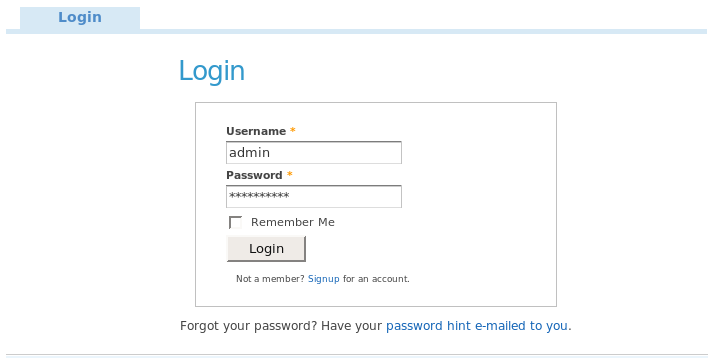
\includegraphics[scale=0.5]{login}
\caption{Login Form}\label{fig:login-page}
\label{fig:login}
\end{figure}

Login with your username and password.

\section{Home Page}
After you have logged in successfully, you will be redirected to your
\emph{home page}. The menu items differ based on the type of the user role. If
logged in as a \emph{manager}, you should see the menu and shortcut links as
shown in Figure~\ref{fig:manager-home-page}. For users with annotator roles,
the number of available options will be reduced (e.g., the menus
\emph{Resources} and \emph{Projects} will not be visible).
\begin{figure}[htb!]
\centering
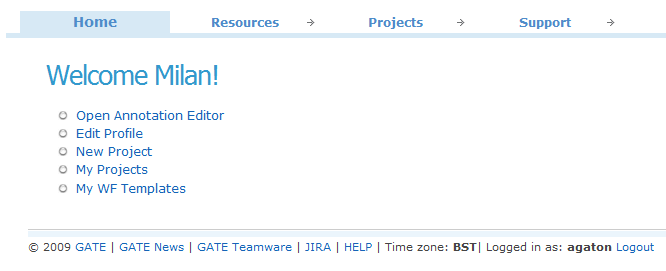
\includegraphics[scale=0.5]{main}
\caption{Home Page - Example}
\label{fig:main}
\end{figure}

\section{Edit Profile}
You can access/change your profile by clicking on \emph{Edit Profile} link from
the home page (see Figure~\ref{fig:main}). The
\emph{Edit Profile} form as shown in Figure~\ref{fig:editprofile}.
\begin{figure}[ht!]
\centering
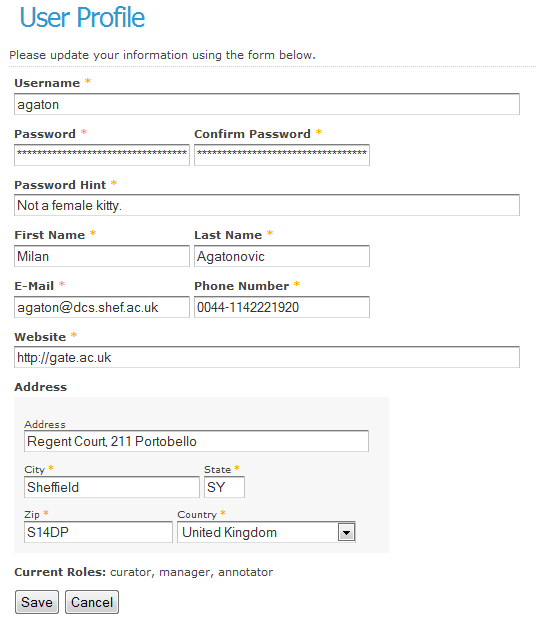
\includegraphics[scale=0.5]{editprofile}
\caption{Edit Profile}
\label{fig:editprofile}
\end{figure}

Note that, in case of AD authentication, only those fields which exist in your
AD profile will be copied to your GATE Teamware profile (see Table~\ref{tab:fields}). Other field values
will be provisional and you should change them after the first login.

\begin{table}[ht!]
\vspace{0mm}
\begin{center}
\caption{The overview of matched fields in AD and Teamware DB}
\vspace{2mm}
\small
\label{tab:fields}
\begin{tabular}{ | l | l |}
\hline
\textbf{Active Directory attribute name} &
 \textbf{Teamware DB Field Name} \\ \hline  \hline

\emph{givenName} & \emph{first\_name}\\
\hline
 \emph{sn} & \emph{last\_name}\\
\hline
 \emph{sAMAccountName} & \emph{username}\\
\hline
\emph{msSFU30Password} & \emph{password}\\
\hline
\emph{mail} &    \emph{email}\\
\hline
\emph{telephoneNumber} & \emph{phone\_number}\\
\hline
  \end{tabular}
\normalsize{}
\end{center}
\vspace{-5mm}
\end{table}

\section{Logout}
When you finish your session, click on \emph{logout} link in the bottom-right
corner.

\chapter{User Management}
\section{Manage Users}
This chapter provides details about user and role management which you can
do if you have \emph{administrator} role. \emph{Manage Users} option from
\emph{Admin} menu will take you to the user list page (see Figure~\ref{fig:userlist}) 
from where you can: add new user(s) (one by one or bulk), view, edit,
enable/disable and delete users.
\subsection{Add Users}
To add a new user click on the \emph{Add}
button\footnote{Please note that newly added users need not to have AD account
before hand}.

\begin{figure}[hb!]
\centering
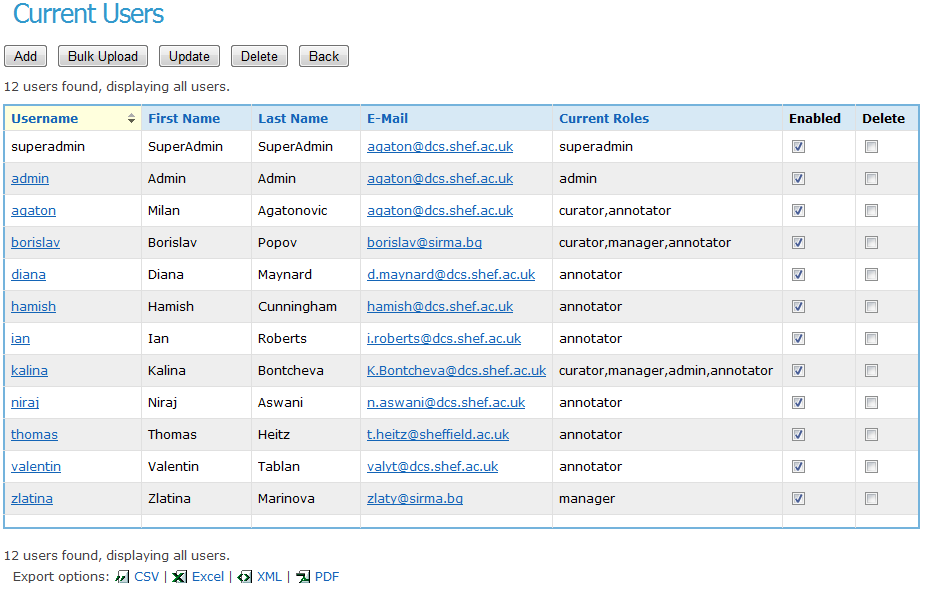
\includegraphics[scale=0.4]{userlist}
\caption{User List}
\label{fig:userlist}
\end{figure}

\subsection{Bulk Users Upload}
To upload multiple users click on
the \emph{Bulk Upload} button.
\begin{figure}[hb!]
\centering
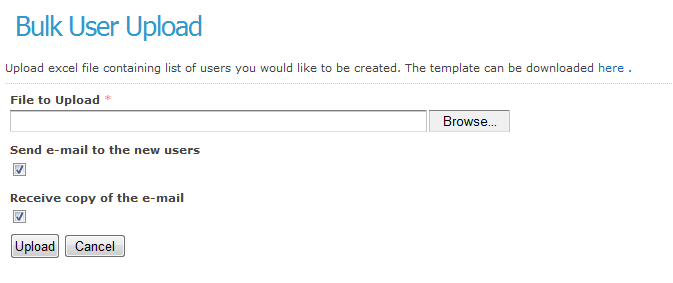
\includegraphics[scale=0.4]{bulkuserupload}
\caption{Bulk Users Upload}
\label{fig:bulkuserupload}
\end{figure}
You can download the excel template file, by clicking on provided link and fill
it with the user data like shown in
Figure~\ref{fig:bulkuseruploadxlstemplate}
If you want users to be notified upon their registration, check \emph{Send
e-mail to the new users}, and if you want yourself to have copy of this email
check \emph{Receive copy of the e-mail}.

\begin{figure}[hb!]
\centering
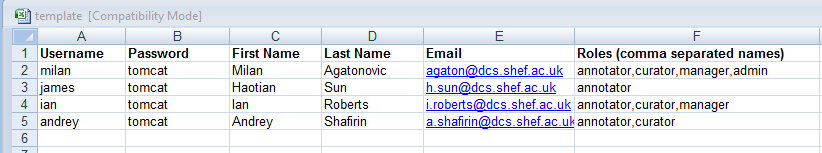
\includegraphics[scale=0.4]{bulkuseruploadxlstemplate}
\caption{Excel Template File}
\label{fig:bulkuseruploadxlstemplate}
\end{figure}

Please note that roles assigned to the new user have to comma separated

\subsection{View/Edit user profiles and roles}
If you want to update the information of the user
\emph{agaton}, he/she can simply click on the username link of
\emph{agaton} shown in Figure~\ref{fig:userlist}.

\begin{figure}[hb!]
\centering
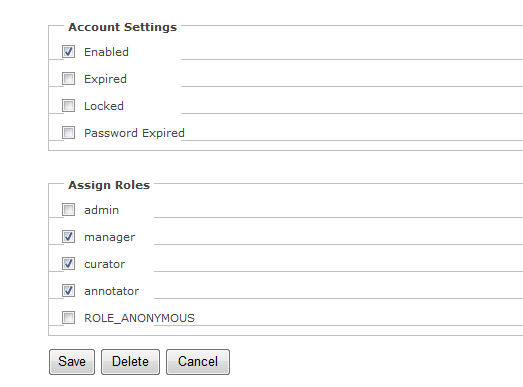
\includegraphics[scale=0.4]{userprofile}
\caption{Edit User Profile}
\label{fig:userprofile}
\end{figure}

The user information form will be displayed. In addition to the information
shown in Figure~\ref{fig:editprofile} previously, this form will be extended
to include details of user roles and account settings as shown in
Figure~\ref{fig:userprofile}. Here administrator can assign multiple
roles to each user.

\subsection{Enable/Disable Users}
You can quickly enable/disable multiple users by
ticking/unticking the checkboxes in the user list \emph{Enabled}, and clicking
on the \emph{Update} button.

\subsection{Delete Users}
You can delete multiple users by
ticking the checkboxes in the user list \emph{Delete} column, and
clicking on the \emph{Delete} button.

\section{Active users}
Who among users is online can be seen from the \emph{Active Users} page as
shown in Figure~\ref{fig:currentuser}.
\begin{figure}[hb!]
\centering
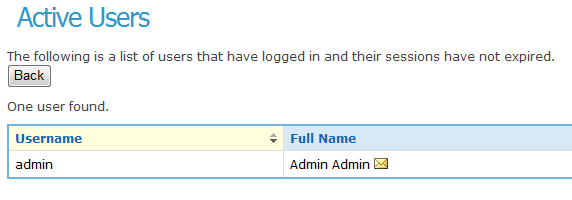
\includegraphics[scale=0.4]{currentuser}
\caption{Active Users}
\label{fig:currentuser}
\end{figure}

\section{Clickstreams}
Administrator can view user request history via \emph{Clickstreams} page, which 
is the last item in the Administration menu, as
shown in Figure~\ref{fig:allclickstreams}.
\begin{figure} [hb!]
\centering

\includegraphics[scale=0.5]{allclickstreams}
\caption{Clickstreams}
\label{fig:allclickstreams}
\end{figure}


\chapter{Resource Management}
In this chapter, we explain how you can manage resources like documents
(corpora), annotation schemas and annotation services if you have a \emph{manager} role.

\section{Corpora}
%GATE Teamware provides means to perform operations in a remote GATE Datastore.

\subsection{Corpora List}\label{section:corpora-list}
To view existing corpora, choose \emph{Resources $>>$ Documents} from the top
menu. New page will be shown with the complete list of available corpora as
shown in Figure ~\ref{fig:corporalist}.
\begin{figure}[htb]
\centering
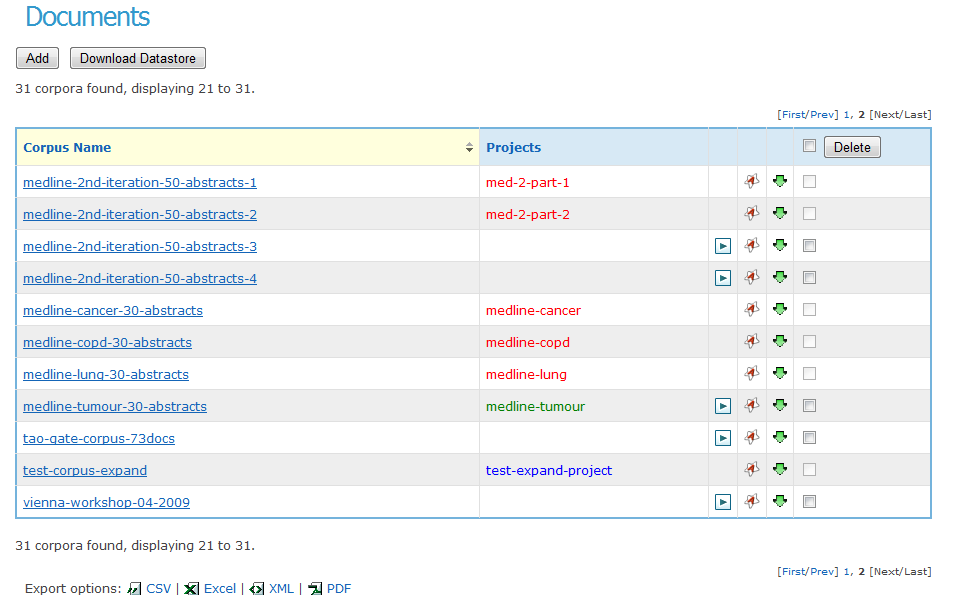
\includegraphics[scale=0.4]{corporalist}
\caption{Copora List}
\label{fig:corporalist}
\end{figure}
From this page, you can choose several
options:
\begin{description}
\item [Modify Corpus] To view details about already existing corpus, click on
the link showing the corpus name, or the first icon in the row. If you want to
add some new documents in corpus, you can do this by clicking on
\emph{Upload Documents} button.
\item [Start Annotation Project] Directly from the corpora list, you can start
annotation project for each corpus, by clicking on the \emph{start} icon. 
The annotation projects will be
explained in details in the next chapter. For now, have this option in mind as
a convenient way to start annotation from this page.

\item [View Annotation Projects] You can see if some annotation project is
running, suspended or finished over each corpus. The links to the annotation
project statistics can be of different colours, depending on project status:
\emph{red}: suspended; \emph{blue}: running; \emph{green}: completed. More about
project statistics you can find in the next chapter.

\item [Download Corpus] If you click on \emph{Download} link (second icon from
the right) you will download the corpus with all documents in it, archived in
zip file.
\item [Download Datastore] If you click on \emph{Download Datastore} button you
will download whole datastore with all corpora, archived as zip file.
\item [Delete Corpus] If you tick the checkbox in \emph{Delete} column (last
column on the right hand side) and press \emph{Delete} button you will delete
selected corpora with all documents in them.
\end{description}

\subsection{Create Corpus}
To create a new corpus, click on the \emph{Add} button on the corpus list page.
New window will open (see Figure ~\ref{fig:addcorpus}). Specify the corpus name
and encoding. By default the
encoding is UTF-8 which should be fine for most of the documents. However if
you need some particular encoding, you should specify it here. Click
\emph{Browse} button to provide the full path of your zip archive from your file
system.

\begin{figure}[h]
\centering
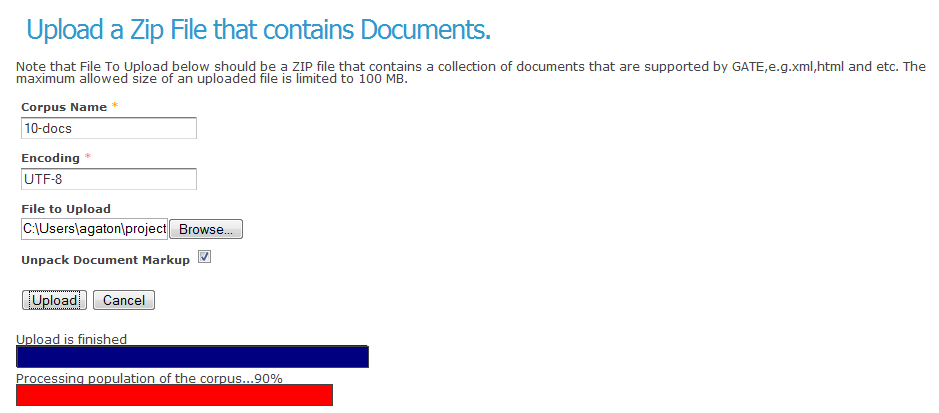
\includegraphics[scale=0.5]{populatecorpus}
\caption{Add Corpus }
\label{fig:addcorpus}
\end{figure}

GATE Teamware will try to identify the type of the document, then strip
and convert any markup into GATE's annotation format. To disable this process,
uncheck the option \emph{Unpack Markup Aware}. Finally click on the
\emph{Upload} button to populate the corpus.

Please have in mind the following conditions:
\begin{itemize}
\item documents need to be packaged in zip archive
%You have nested folders in zip archive.
\item documents have to be in a format supported by GATE:
Plain Text, HTML, SGML, XML, RTF, PDF, DOC or XLS
	
\end{itemize}
\begin{figure}
If the corpus is populated successfully, you should see a screen similar to the
one shown in Figure \ref{fig:corpuspopulated}.
\centering
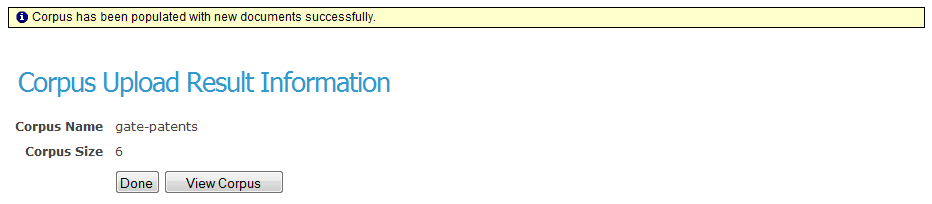
\includegraphics[scale=0.4]{corpuspopulated}
\caption{Corpus created}
\label{fig:corpuspopulated}
\end{figure}

Please make sure that the zip archive you are uploading is created by standard
zip archiver tool and that compression method used is
DEFLATE\footnote{\url{http://en.wikipedia.org/wiki/DEFLATE}}. There should be no
problem with standard zip implementation under Windows and Unix.
In case you get the error message like in Figure
\ref{fig:unsupportedcompressionmethod},
try to zip your corpus with the different tool.
\begin{figure}
\centering
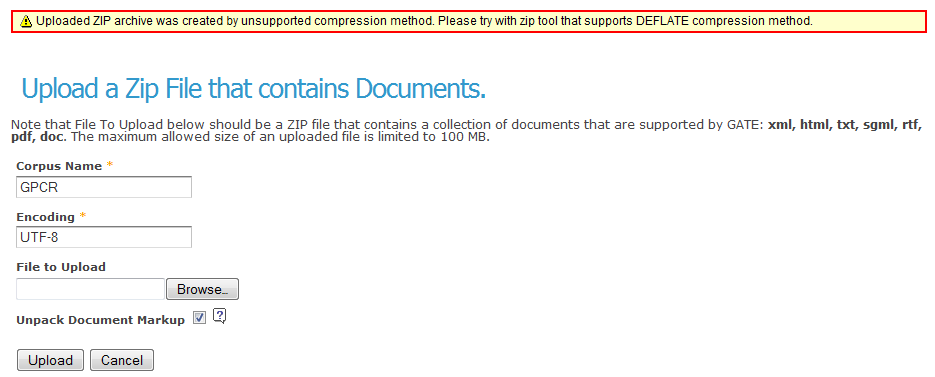
\includegraphics[scale=0.4]{unsupportedcompressionmethod}
\caption{Unsupported Compression Method}
\label{fig:unsupportedcompressionmethod}
\end{figure}

\subsection{ANNIC Search}
To use ANNIC Search facility, click on the ANNIC icon for the corpus you want
to carry out the search. A Java Web Start application - ANNIC GUI will be
activated. 

\begin{figure}[hb!]
\centering
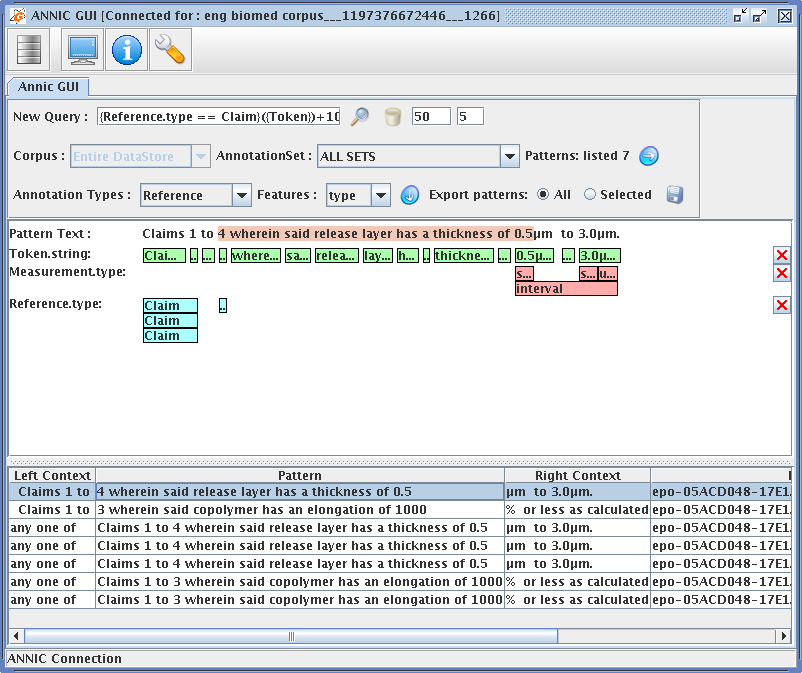
\includegraphics[scale=0.4]{annicresult}
\caption{Annic Search Result}
\label{fig:annicresult}
\end{figure}

The Figure  ~\ref{fig:annicresult} shows ANNIC
in action. Since ANNIC allows indexing documents
with annotations and features, the syntax of ANNIC query contains LHS part
of the JAPE pattern/action rule.



For example, the query:
${Reference.type == Claim}({Token})+10{Measurement}$ will find first an
annotation of type \emph{Reference} that has a feature named type with the value
\emph{Claim}, then to allow from 1 to 10 annotations of type \emph{Token}, i.e.
a word or punctuation, and eventually to find an annotation of type
\emph{Measurement}. This query can be interpreted as a search for finding a
reference to a claim that involve measurement.

To execute a query, enter it in the query text field, and click
on the magnifying glass icon. You can choose annotation sets,
then the annotation type, and features to add to the middle part of the
GUI with the bottom arrow icon. If there is more than one page of results
you need to use the right arrow icon to see the next page of results.

You can see the results in the bottom part of the GUI that lists in a
table the matching patterns, their contexts, the name of the document
and annotation set. In the middle part, you can see the annotations
and features with their values for the line selected in the bottom part.

Help window is provided in the GUI if you click on the information
sign icon in the top tool bar. For more information about Annic and JAPE, please
check Gate User Guide.

\section{Documents}
\subsection{Document list}
To see the list of documents inside the corpus click on \emph{View} link next
to the corpus name. New page will open as shown in
Figure ~\ref{fig:documentlist}.
\begin{figure}[h]
\centering
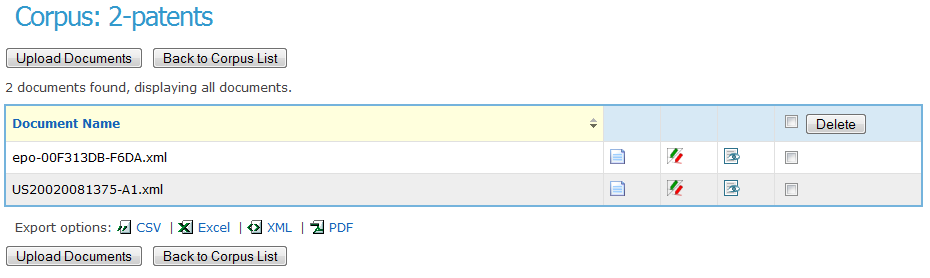
\includegraphics[scale=0.5]{documentlist}
\caption{Document List}
\label{fig:documentlist}
\end{figure}

To delete a document from the corpus, simply tick the checkbox next to document
and click on the
\emph{Delete button}. You can choose to delete all listed documents by ticking
the box from the top of the table.

\subsection{View Document with Annotation Editor}\label{section:annotation-editor}
To open/edit a specific document, click on the \emph{View Document} icon (the
first icon from the left hand side shown in Figure~\ref{fig:documentlist}).
Annotation Editor will be activated and start
loading the document. As shown in Figure ~\ref{fig:annotatorgui}, users can
now carry out the annotation tasks within the Annotator GUI.

\begin{figure}[ht!]
\centering
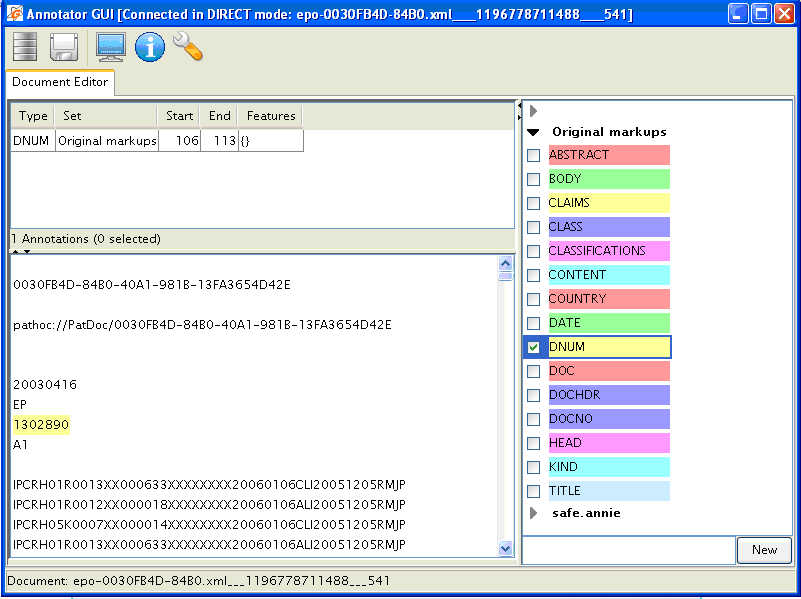
\includegraphics[scale=0.35]{annotatorgui}
\caption{Annotation Editor}
\label{fig:annotatorgui}
\end{figure}

\subsection{Compare Annotations with Annotation Differ}\label{section:annotation-differ}

To use the Annotation Differ facility on the document, click on the icon
\emph{Annotation Differ} on the documents list page (the second icon from the
left hand side shown in Figure ~\ref{fig:documentlist}). Then, you should see the
Annotation Diff Editor, where you need to specify which two annotation sets
and the common annotation type you want to compare.

\begin{figure}[hb!]
\centering
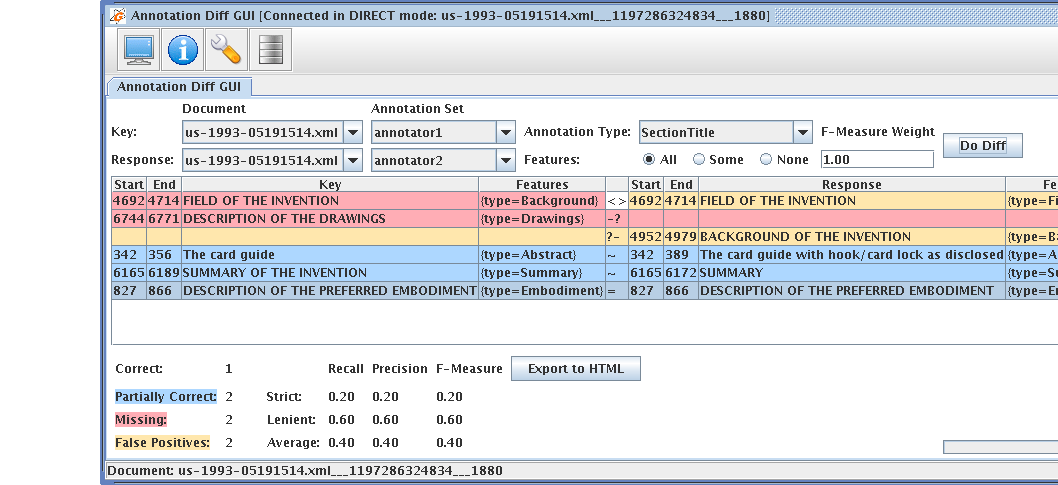
\includegraphics[scale=0.32]{anndiffgui}
\caption{AnnDiff Editor}
\label{fig:anndiffgui}
\end{figure}

Figure ~\ref{fig:anndiffgui} depicts a comparison
between two annotators who have their annotations contained respectively in
\emph{annotator1} and \emph{annotator2} annotation sets. The first is the key,
i.e. the gold standard, and the second is the response, i.e. the tested data.
There is a common annotation type \emph{SectionTitle} in these annotation sets.
It is thereby possible to do a comparison on this annotation type.

The option \emph{Features} has been set on \emph{All} -- this means that all
values of the
features are taken into account during comparison. For example, the first
line in the table shows for the same text, \emph{Field of invention}, two
different feature values, \emph{Background} and \emph{Field} for the same
feature named \emph{type}.

You can see different colors according to the type of difference between the
annotations from each annotation set that is also shown in the central column
of the table.

Help window is provided in the GUI if you click on the information sign icon
in the top tool bar. For more information, please refer to the \emph{Chapter 13},
Performance Evaluation of Language Analysers, in Gate User Guide
(\url{http://www.gate.ac.uk/sale/tao/index.html}).

\subsection{IAA Calculation}
From the document list page, you can do IAA calculation over annotation sets on
each document. Click on the IAA icon (third icon from the left hand side shown
in Figure~\ref{fig:documentlist}), and the new page should open as shown in
Figure~\ref{fig:iaacalculation}.
\begin{figure}[ht!]
\centering
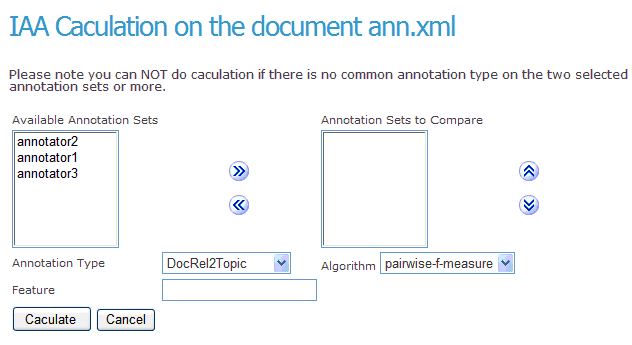
\includegraphics[scale=0.4]{iaacaculation}
\caption{IAA Calculation}
\label{fig:iaacalculation}
\end{figure}

You need to select at least two annotation sets from the left available
annotation sets box and move them to the right box to do the comparison over a
shared annotation type. Also there are four algorithms available for you to choose.
The screenshot shown in Figure ~\ref{fig:iaaresult} is an example of the result
based on the chosen annotation sets, type and algorithm. Note: four algorithms
offer different result formats because of their difference in various values.

\begin{figure}[h!]
\centering
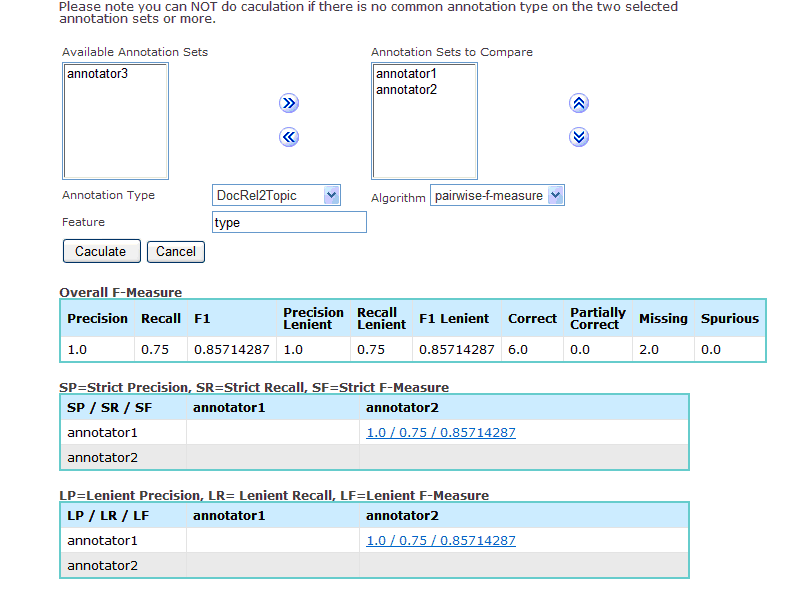
\includegraphics[scale=0.4]{iaaresult}
\caption{IAA Calculation Result}
\label{fig:iaaresult}
\end{figure}

\clearpage
\section{Annotation Schemas}
Users can upload their annotation schemas in XML format to the server so that 
they can be used in the process of manual annotation. Click on the 
$Resources >> Annotation Schemas$ option from the top menu and you will reach 
the annotation schema list page, as shown in Figure~\ref{fig:annoschemalist}.
\begin{figure}[ht!]
\centering
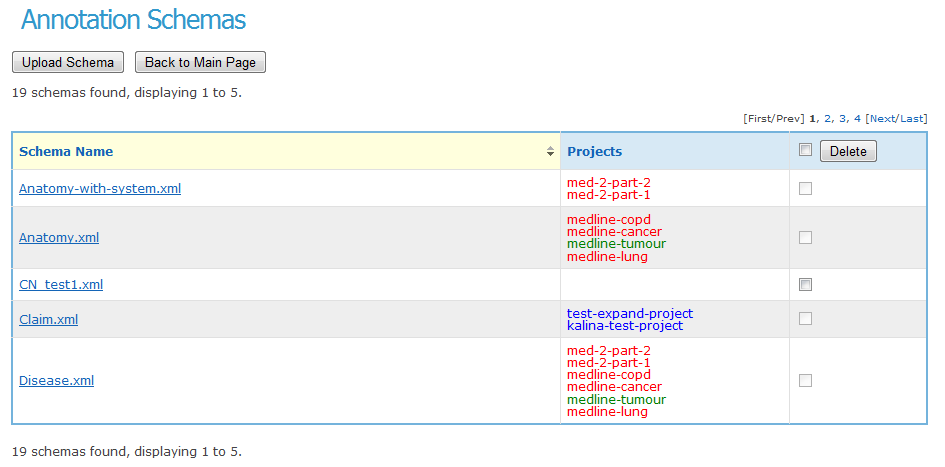
\includegraphics[scale=0.4]{annoschemalist}
\caption{Annotation Schema List}
\label{fig:annoschemalist}
\end{figure}

You can see if some annotation project, using particular schema is
running, suspended or finished. The links to the annotation
project statistics can be of different colours, depending on project status:
\emph{red}: suspended; \emph{blue}: running; \emph{green}: completed. More about
project statistics you can find in the next chapter.

To upload a new annotation schema to the server, click on the 
\emph{Upload Schema} button and you should reach the page where you can 
select the schema file on your file system (see Figure ~\ref{fig:addschema}).
\begin{figure}[ht!]
\centering
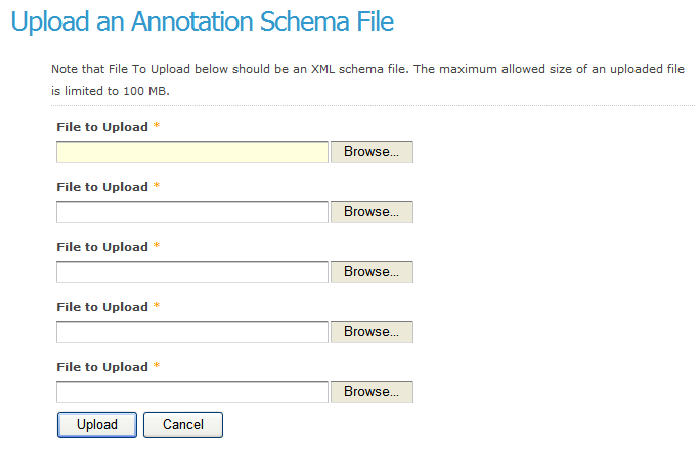
\includegraphics[scale=0.4]{addschema}
\caption{Upload Annotation Schema}
\label{fig:addschema}
\end{figure}

After clicking on the \emph{Save} button from , you will see
the confirmation message and the annotation schema you have added.

To delete one or more schemas, check the tickbox in the last column of the 
table (see Figure ~\ref{fig:annoschemalist})  and click \emph{Delete}. 

If you want to view annotation schema click on \emph{View} icon.

\section{Annotation Services}
Users with \emph{Administrator} role can view, add, update, and delete
annotation services. To view available annotation services, select
\emph{Services} option from \emph{Resources} menu
(see Figure~\ref{fig:annotationservices} below).
\begin{figure}[hb!]
\centering
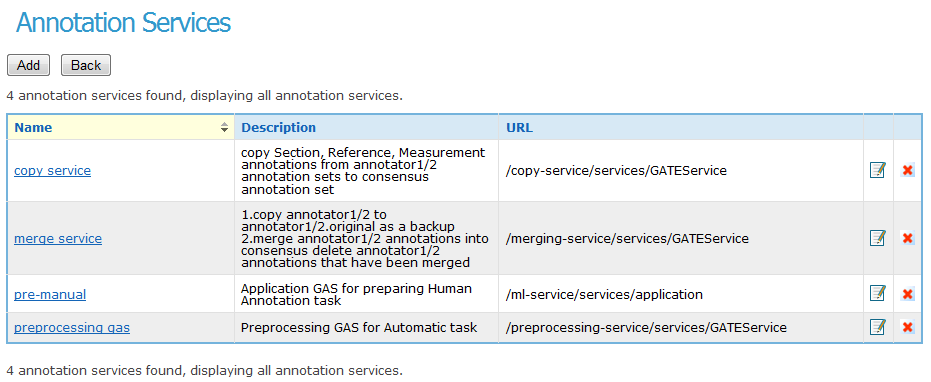
\includegraphics[scale=0.4]{annotationservices}
\caption{Annotation Services}
\label{fig:annotationservices}
\end{figure}

Here you can delete or update existing annotation services or create a new one.
Note that currently, GATE Teamware supports only GATE services (GAS).

To create a new GAS service, click on \emph{Add} button and fill in the form as
shown in Figure~\ref{fig:createannotationservice}.
\begin{figure}[hb!]
\centering
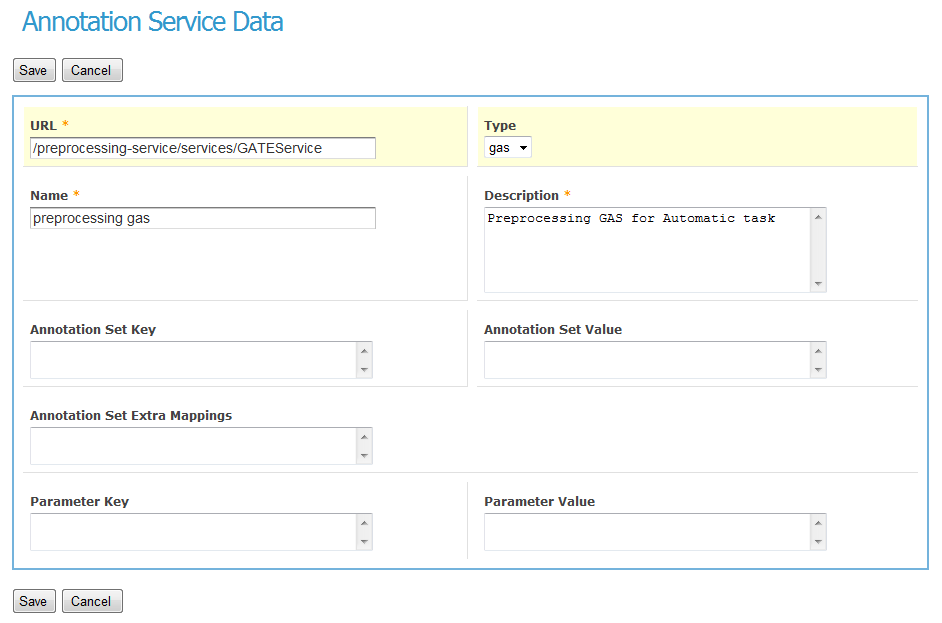
\includegraphics[scale=0.38]{createannotationservice}
\caption{New Annotation Service}
\label{fig:createannotationservice}
\end{figure}

This form is used to inform Teamware about a published service -- the service
must already be deployed at a URL accessible to the Teamware server.  The GATE
user guide\footnote{\url{http://gate.ac.uk/userguide/sec:howto:export}}
explains how to save a GATE application in a suitable package for publishing as
a Teamware service.
%
% When we have tools to automate the zip -> war step, this section will need to
% be expanded, it is deliberately vague at the moment...
%

Mandatory fields are:
\begin{itemize}
  \item \emph{url}: the URL of the GAS service you have published;
  \item \emph{name}: the friendly title, you will refer to, when you
configure your \emph{Workflow Template};
  \item \emph{description}: a few words about what GAS is doing.
\end{itemize}

It is important to mention that if you ommit \emph{http} in the
URL, it will be assumed that GAS is published under the same context as the web
application.
For example on Figure~\ref{fig:createannotationservice}, the preprocessing-gas
has URL
\emph{/preprocessing-service/services/GATEService}. That means if GATE Teamware
is hosted on
\emph{http://somehost/teamware} the GAS URL will be resolved as:
\emph{
http://somehost/teamware/preprocessing-service/services/GATEService}.






\chapter{Project Management}
\section{Introduction}
\emph{Project Management} functionality is accessible to the \emph{manager} and \emph{administrator} roles
only. Managers can access and modify content created by themselves only, while administrators can see and edit all content available in the system.

From the home page you
can either use available shortcuts, or you can access even more options from the
\emph{Projects} menu on the top. As a manager you will see options as shown in
Figure~\ref{fig:manager-home-page}, while as an administrator you will see more options (see Figure~\ref{fig:admin-home-page}).

\begin{figure}[htb]
\centering
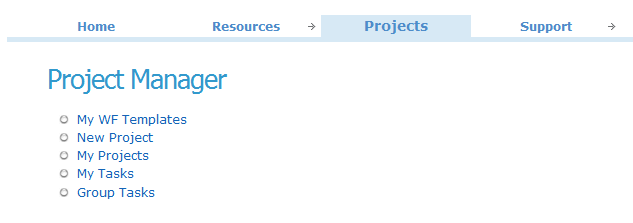
\includegraphics[scale=0.5]{manager-home-page}
\caption{Project menu for \emph{managers}}
\label{fig:manager-home-page}
\end{figure}

\begin{figure}[htb]
\centering
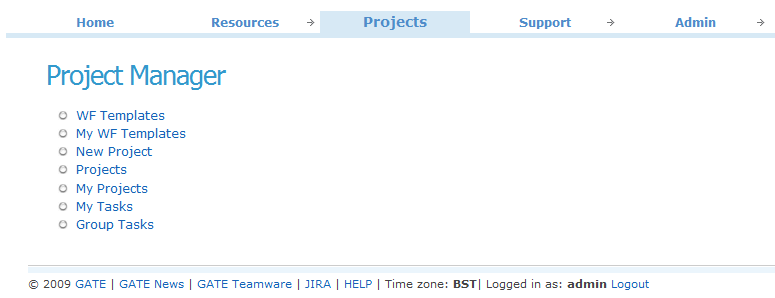
\includegraphics[scale=0.5]{admin-home-page}
\caption{Project menu for \emph{administrators}}
\label{fig:admin-home-page}
\end{figure}


\emph{Annotation projects} are meant to support the following annotation
modules: 

 \begin{itemize}
   \item \emph{automatic}
   \item \emph{manual}
   \item \emph{post-manual (consensus)}
   \item \emph{review}
   \item \emph{post-processing (final consensus)}
 \end{itemize}

You can use any particular module or all of them in the predefined order.
If you want use \emph{manual} or \emph{review} module, you will be able to manage
annotators and curators and specify annotation rules. 

In case of \emph{automatic}, \emph{post-manual}  or \emph{post-processing} 
mode you can choose from existing GATE services (GAS) which can be executed in
sequence. Please see the \emph{Annotation Services} chapter for more details. 

The motivation for combining all modules is to use pre-processing to
bootstrap the manual annotation process. The result of
manual annotation result is consolidated by using post-manual module, in other
words the annotation sets created by human annotators, e.g. \emph{annotator1/2}
are inspected and merged. The identical annotations are moved to \emph{consensus} annotation set and the
different ones are left in \emph{annotator1/2}.
Review process should validate the annotations in \emph{annotator1/2} and
delete false ones. This will leave only reviewed annotations in
\emph{annotator1/2}.

Finally, the remaining - valid annotations in \emph{annotator1/2} are copied to
\emph{consensus} set by post-processing module.

\section{Create new WF template}\label{section:create-new-template}
To create new project, it is mandatory to create Workflow (WF) template first.
Templates are later accessible for creating similar projects.

To create new template, you need to choose \emph{Projects $>>$
My WF Templates $>>$ Create New WF Template with Wizard} option from the top
menu. The wizard will then
guide you through the process of creating template as explained next in Section
~\ref{section:workflow-template-wizard}.

Another way to create new template is during the creation of New project (
explained later in Section
~\ref{section:create-new-project}) by selecting option
\emph{Blank template} at the list of available templates. Click \emph{Select}
button, and you will be redirected to the \emph {Workflow Template} page, from
where you are entering \emph {Workflow Template Wizard}.

\subsection{Workflow Template Wizard}
\label{section:workflow-template-wizard}
\begin{figure}[hb!]
\centering
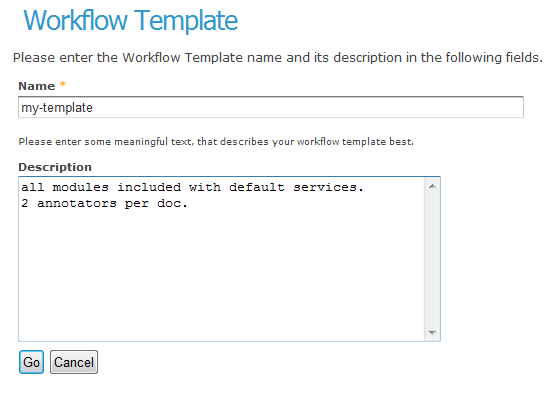
\includegraphics[scale=0.4]{createwftemplate}
\caption{Create New Workflow template}
\label{fig:createwftemplate}
\end{figure}
You need to provide the \emph{name} and \emph{description} of the template.
These two fields will be later used to show overview of the templates and therefore should
contain useful information to help you distinguish between various templates.
Click \emph{Go} button as shown in Figure~\ref{fig:createwftemplate}).

The wizard comprises several steps, the number of which is not fixed as
each of them depends on the preselected options in the previous step.

\begin{figure}[htb]
\centering
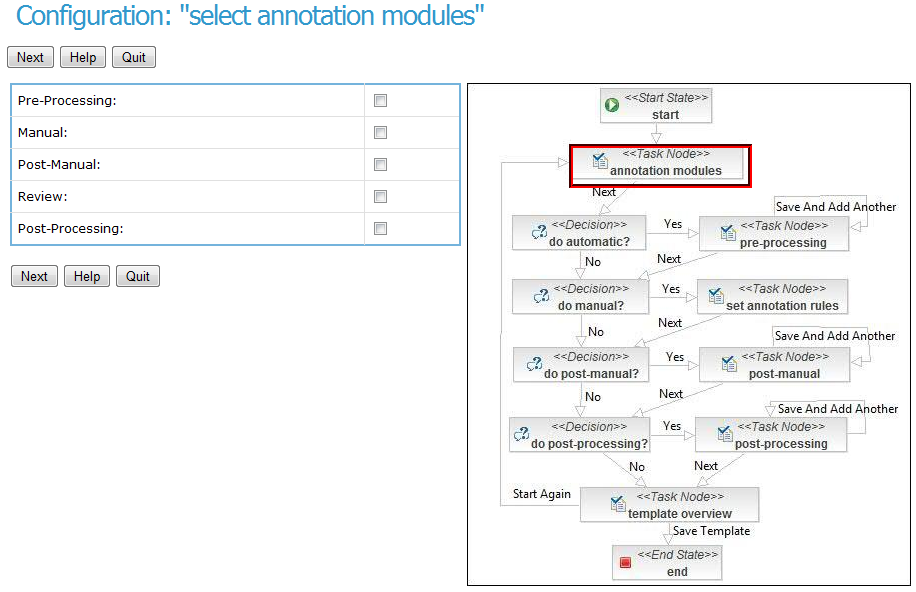
\includegraphics[scale=0.4]{selectannotationmodes}
\caption{Configuration: Select Annotation Modules}
\label{fig:selectannotationmodes}
\end{figure}

During the wizard, the \emph{progress diagram} on the right hand side will
show your progress by highlighting your current step.

The first step is the \emph{Configuration: "select annotation modules"} step,
where you need to choose one or more annotation modules: \emph{automatic},
\emph{manual}, \emph{post-manual}, \emph{review} and/or
\emph{post-processing}, as shown in Figure~\ref{fig:selectannotationmodes}).

Click \emph{Next}. Depending on the chosen modules, the steps to follow
will vary. Here is the detailed explanation of each possible step in case when
all available modules are selected.
\begin{description}
   \item [Pre-processing:] To configure \emph{pre-processing} you need to select
   one or more pre-processing services. When you are done with selection press 
   \emph{Next}. Alternatively you can add as many services as you want to 
   the pipeline by clicking on the button \emph{Save and add another}. This step
  is shown in Figure~\ref{fig:gaspreprocessing}). 
\begin{figure}[hb!]
\centering
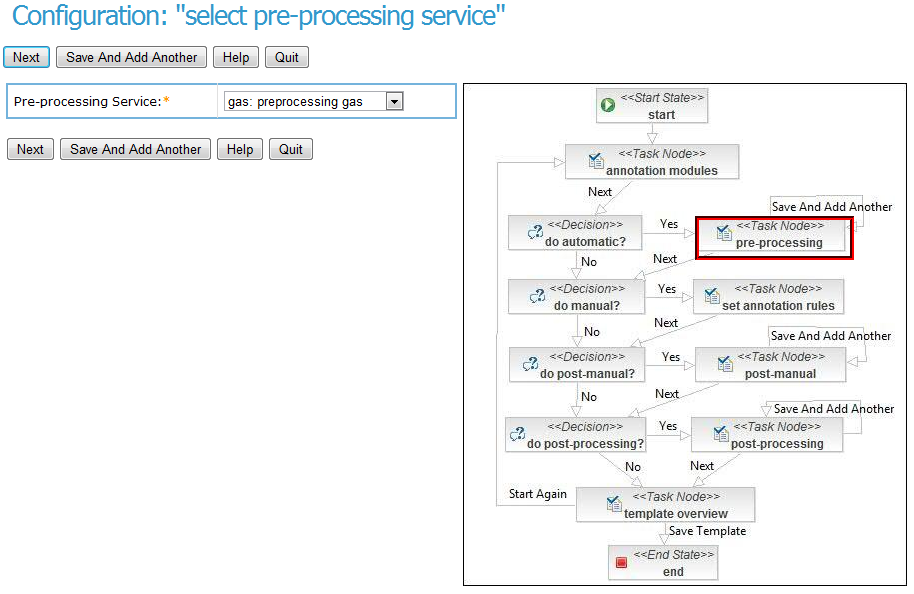
\includegraphics[scale=0.4]{gaspreprocessing}
\caption{Configuration: GAS Pre-processing}
\label{fig:gaspreprocessing}
\end{figure}
    \item  [Manual annotation:] Manual annotation needs a few parameters to be
    specified. This is done in the \emph{Configuration step: "select annotation rules"} 
    as shown inFigure~\ref{fig:selectannotationrules}. Here you will need to:
   \begin{itemize}
       \item select number of annotators per document. For example if you select
       2, each document should be annotated by 2 different annotators;
       \item leave \emph{cancel task allowed} checked; this will allow
       annotators to cancel tasks if they feel unsure about how to annotate the
       document correctly;
       \item leave \emph{anonymous annotation} checked; this will create
       generic annotation set names for annotators (e.g., \emph{annotator1},
       annotator2, etc.) instead of using their usernames. This option is
       useful when you later search annotation sets within documents in
       generalised fashion (for example, using regular expression 'annotator*');
       \item select some of the existing annotation schemas which will be
       loaded inside the Annotation Editor during the process of manual
       annotation (you also have the option to add new schema, if you want).
       \item choose the service which will prepare manual annotation task 
       (copy preprocessed annotations into annotator's annotation set)
   \end{itemize}
 \item  [Post-Manual: and Post-Processing] In \emph{Configuration steps:
   "select post-manual service"}, you can select one or more
   post-manual/post-processing services as shown in
   Figure~\ref{fig:selectpostmanual}. These steps are identical to
   \emph{pre-processing}. The main point is that you can chain services in the order you like 
   and make them executed in a pipeline.
\begin{figure}
\centering
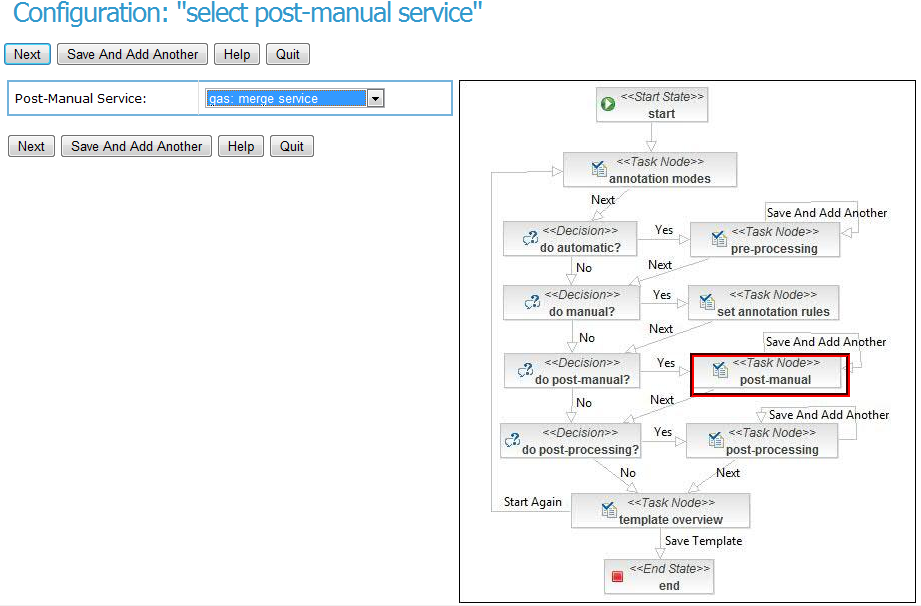
\includegraphics[scale=0.38]{selectpostmanual}
\caption{Configuration: Select Post-Manual}
\label{fig:selectpostmanual}
\end{figure}
\end{description}


From the \emph{Configuration: "template overview"} page
(Figure~\ref{fig:templateoverview}) the template can be saved by clicking on the
\emph{Save template} button. You will be redirected to the
 \emph{My WF Templates} page. Note that if you are not happy with the settings,
 you can repeat the setup procedure by pressing \emph{Start Again} button.
\begin{figure}
\centering
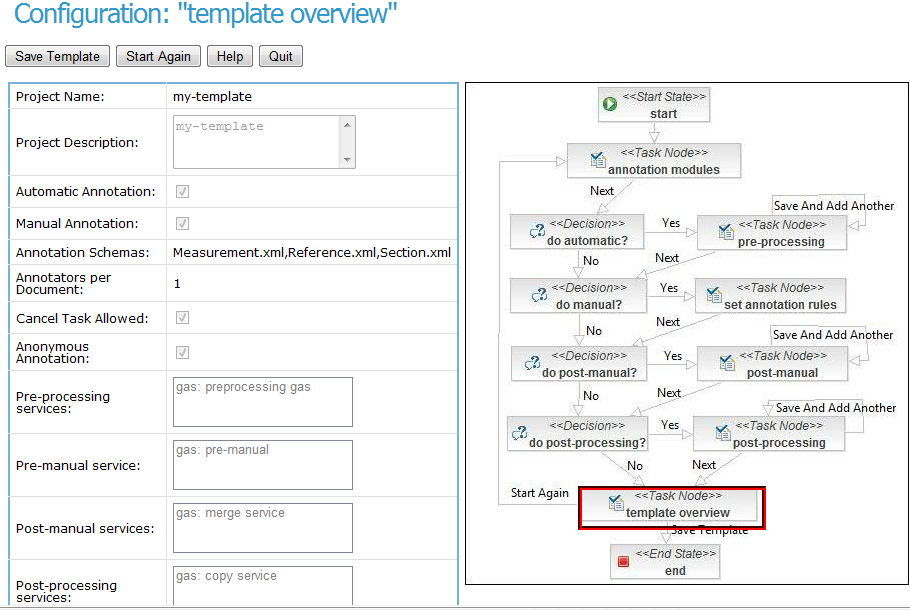
\includegraphics[scale=0.38]{templateoverview}
\caption{Configuration: Template Overview page}
\label{fig:templateoverview}
\end{figure}

At any time you can get more information on the current step or instructions
on how to proceed by hovering over the
 \emph{Help} button. This is especially useful in cases when you are not
sure on how to complete the step.
Quitting the wizard is always possible by pressing the \emph{Quit}
 button. After the warning, and choosing the option \emph{Yes}, the wizard will
 exit, but it can be resumed any time by selecting \emph{Projects $>>$ My WF
 Templates}, and then by clicking \emph{Resume} button for the selected
 template.



\section{My WF templates}\label{section:wf-templates}
Choose \emph{Projects Menu $>>$My Workflow Templates} option from the top menu
or \emph{My Workflow Templates} link at your home page.
You will enter \emph{My WF Templates} page as shown in Figure
~\ref{fig:mywftemplates}.
\begin{figure}[htb]
\centering
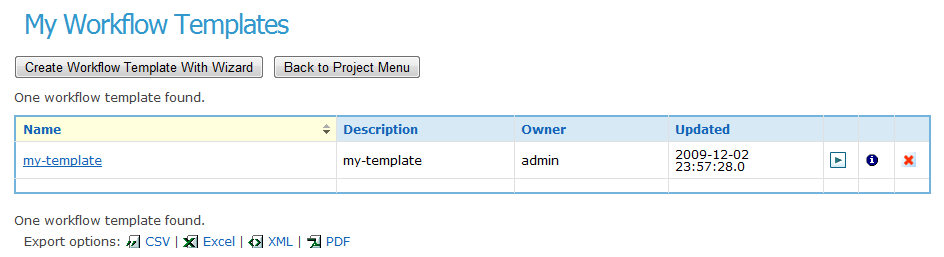
\includegraphics[scale=0.4]{mywftemplates}
\caption{My Workflow Templates}
\label{fig:mywftemplates}
\end{figure}
As we have mentioned previously in Section~\ref{section:create-new-template},
you will land on this page after finishing wizard successfully. In this case,
the status of workflow template will be \emph{Ready}, meaning that you can
create project based on this template (the \emph{Create Project} icon will be
visible only if the template is ready). If during the wizard you quit the
process before finishing template setup, the status of the template will be
\emph{Not Configured}. By clicking on \emph{Resume} icon, you will be able to
resume the setup and complete unfinished steps.

If you want to delete a \emph{Workflow Template}, you can do so by clicking on
the \emph{Delete} icon. Note that all projects based on selected template will
be deleted.

Of course, you will often need to check what configuration is saved in template.
This can be done by hovering \emph{I} icon.

\section{Create new project}\label{section:create-new-project}

For your convenience, there are several ways to create project.
Two have been already mentioned:
 \begin{itemize}
   \item from the corpora list page, you can create project for the specified
corpus by clicking on \emph{Start Project} icon (see
Section~\ref{section:corpora-list}).
   \item from the My Workflow Templates page, you can create project for the
specified template by clicking on \emph{New project} icon (see
Section~\ref{section:wf-templates}).
 \end{itemize}
 
 Here we will cover other ways.
 
From the top menu select "Projects" $>>$ "New Project", or access it 
  directly from the home page. You will be redirected to \emph{Create New 
  Project} page where you need to choose \emph{WF Template}. Here
  you have two options (see Figure~\ref{fig:createnewproject}):
  \begin{itemize}
    \item Choose from the list of available templates and click \emph{Select}.
    \item Create new template, by selecting option \emph{Blank template}.
    If you choose this option, you will need to follow the steps explained
    in Section ~\ref{section:create-new-template}. 
    After you have finished creating the template, you will be redirected to
    the list of WF templates.
  \end{itemize}
\begin{figure}[htb]
\centering
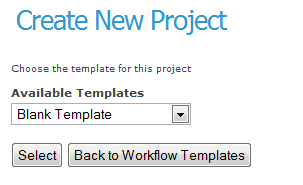
\includegraphics[scale=0.35]{createnewproject}
\caption{Create New Project}
\label{fig:createnewproject}
\end{figure}
You will be redirected to the \emph{Project Data} page where you need to 
provide details of the project. Requested details vary depending on the
annotation modes defined in the WF template. In case you excluded manual
annotation mode, the three options will need to be selected (see
Figure~\ref{fig:projectdata}): project name,
corpus, and manager (you will be selected by default); as a manager of the
project you will be able to see this project in \emph{My projects} list and
manage it (e.g., change actors, monitor project).
\begin{figure}[h!]
\centering
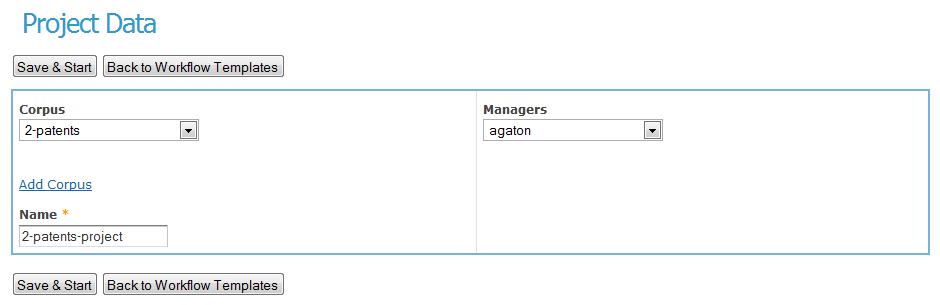
\includegraphics[scale=0.34]{projectdata}
\caption{Configure Project without Manual Annotation}
\label{fig:projectdata}
\end{figure}

When \emph{manual annotation} module is defined, there will be two options in
addition to the previously selected ones: curators and annotators
(see Figure~\ref{fig:projectdatamanual}).
\begin{figure}[htb]
\centering
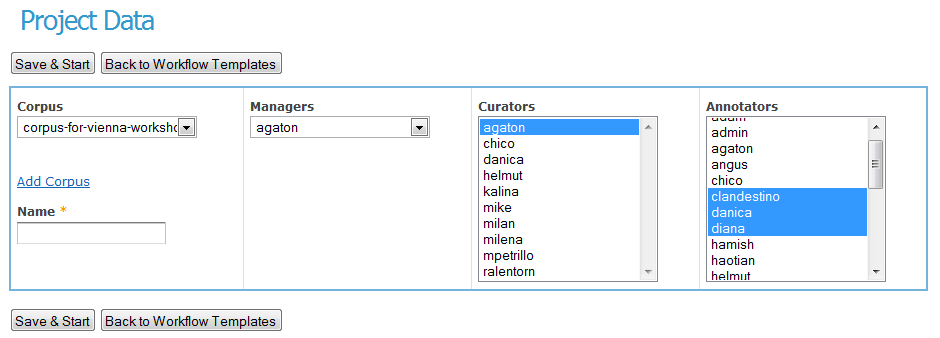
\includegraphics[scale=0.34]{projectdatamanual}
\caption{Configure Project with Manual Annotation}
\label{fig:projectdatamanual}
\end{figure}
For example, you can leave yourself as \emph{manager} and \emph{curator}, and
you can select as many annotators as you wish in the list (hold Ctrl while
selecting annotators for multiple selection of actors).

On the other hand, if you chose \emph{review} module and ommit \emph{manual
annotation} module, there will be an option to select only curators and manager,
since annotators do not take part in review process.

Click \emph{Save \& Start} button and the annotation project will be started.

\section{Annotation Tasks}\label{section:annotation-tasks}

If used template contains manual annotation module all annotators should be
able to get annotation tasks after logging in and clicking on \emph{Open Annotation Editor} from the home page.
We now discuss how annotators (users with \emph{annotator} role execute their
tasks and annotate documents.

As a general rule, users with \emph{Annotator} role assigned, participate in
the project via annotation editor. The annotator's home page contains restricted
operations as shown in Figure~\ref{fig:annotatorhomepage}. The annotator can
either open Annotator editor, or edit his/her profile.
\begin{figure}[htb]
\centering

\includegraphics[scale=0.4]{annotatorhomepage}
\caption{Annotator Home Page}
\label{fig:annotatorhomepage}
\end{figure}

After clicking on \emph{Open annotation editor} link, the annotator has to ask
for the new task. To do this, s/he needs to click on the \emph{Get New Task}
button (the first one from the left side).
Annotation Editor will start to search for available tasks and the annotator
will see the dialogue similar to one shown in
Figure~\ref{fig:getnewtaskineditor}.
\begin{figure}[htb]
\centering
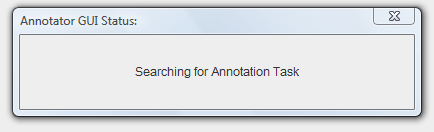
\includegraphics[scale=0.4]{getnewtaskineditor}
\caption{Searching for a new task in Annotation Editor}
\label{fig:getnewtaskineditor}
\end{figure}

If there is an available task, it will be loaded in annotation editor.
The following actions are available (see Figure
~\ref{fig:annotationtaskineditor}):
\begin{itemize}
  \item Finish task (click on the second button from the left) when you finished
with annotations.
  \item Save task (click on the third button from the left) when you want to
save your annotations, but not finish the task.
  \item Reject Task (click on the fourth button from the left) when you feel
unsure how to annotate document and want this to be assigned to other annotator.
\end{itemize}

\begin{figure}[htb]
\centering
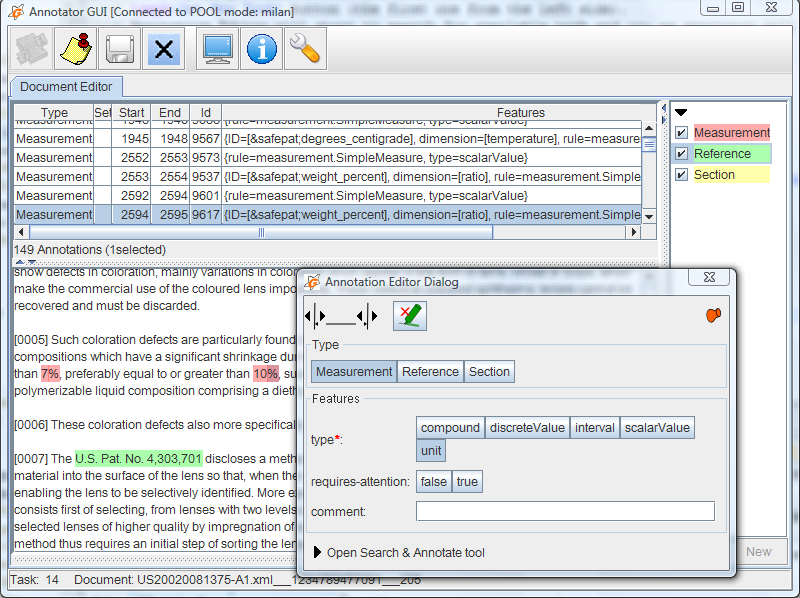
\includegraphics[scale=0.4]{annotationtaskineditor}
\caption{Get New Task in Annotation Editor}
\label{fig:annotationtaskineditor}
\end{figure}

\section{Curation Tasks}\label{section:curation-tasks}
If used template contains \emph{review} module all chosen curators (remember,
you had to select them during project startup) should be able to get curation
tasks after logging in and clicking on \emph{Group Tasks} from the
\emph{Projects Menu} likd shown in Figure~\ref{fig:curator-home-page}. 
\begin{figure}[htb]
\centering
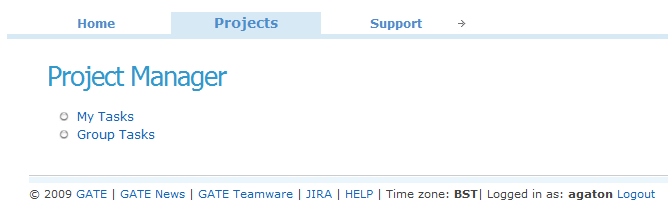
\includegraphics[scale=0.5]{curator-home-page}
\caption{Project menu for curators}
\label{fig:curator-home-page}
\end{figure}

Now we will explain how curator claims and executes his/her tasks and review
documents.

In general, users with \emph{Curator} role assigned, participate in
the project through task form. Since, more than one curator can be assigned to
a particular project, it is necessary for curator to claim his/ger task first,
by clicking on \emph{Accept} icon (see Figure~\ref{fig:reviewgrouptask}). 

\begin{figure}[htb]
\centering
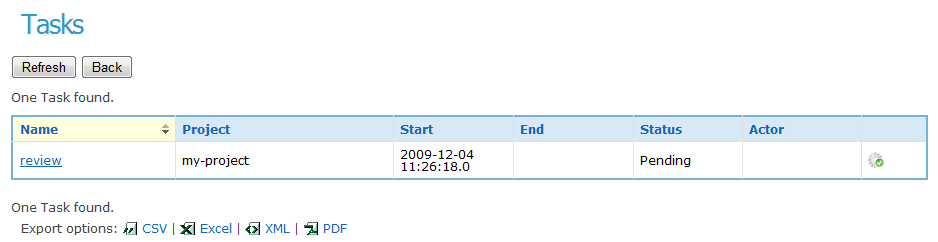
\includegraphics[scale=0.5]{reviewgrouptask}
\caption{Group Tasks}
\label{fig:reviewgrouptask}
\end{figure}

That task will be moved then from \emph{Group Task List} to his/her
\emph{Personal Task list}, as shown in Figure~\ref{fig:acceptedreviewtask} 

\begin{figure}[htb]
\centering
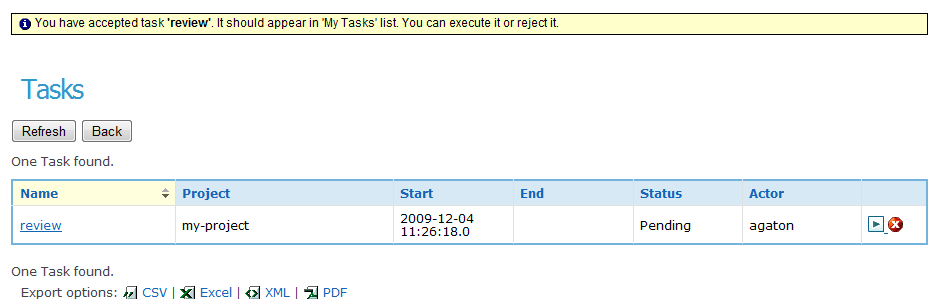
\includegraphics[scale=0.5]{acceptedreviewtask}
\caption{My Tasks}
\label{fig:acceptedreviewtask}
\end{figure}

Curator then executes the task by clicking on \emph{Start} icon.
He will be shown the task form with the instructions which he/she needs to
follow - Figure~\ref{fig:reviewtask} 

\begin{figure}[htb]
\centering
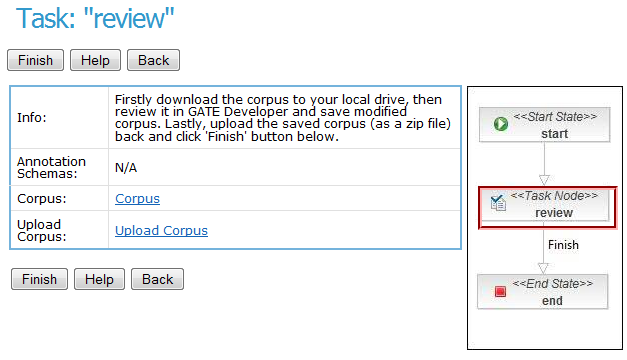
\includegraphics[scale=0.5]{reviewtask}
\caption{Review Task}
\label{fig:reviewtask}
\end{figure}. 

The review procedure briefly comprises the following steps:

\begin{itemize}
  \item Download corpus you need to review as a zip archive, by clicking on
  \emph{Corpus}
  \item Unpack the zip archive and copy documents somewhere on your hard drive
  \item Launch GATE Developer, create new corpus and populate it with the
  unzipped documents.
  \item Run Corpus QA tools (IAA, Annotation Diff, etc) to find out to which
  extent how annotators agree. Note that Corpus QA Tools are added in GATE 5.1.
  \item Delete annotations that you consider false from human annotation sets,
  e.g. \emph{annotator1/2}.
  \item Go back to Teamware, find your task among \emph{My Tasks} and update the
  documents in corpus by clicking on \emph{Upload Corpus} link.
  \item Press \emph{Finish} button in your task form.
\end{itemize}

As a manager you will have more responsibilities than curators and annotators.
One, especially worth mentioning is that managers will be able to manage
projects and have insight into the project progress at any time. In the
following sections we will provide more details on this.

\section{My Projects}
To manage project, select \emph{Projects $>>$ My Projects} from the top menu.
You will see the list of projects that you have created/started, as shown in
Figure~\ref{fig:myprojects}.
\begin{figure}[htb!]
\centering
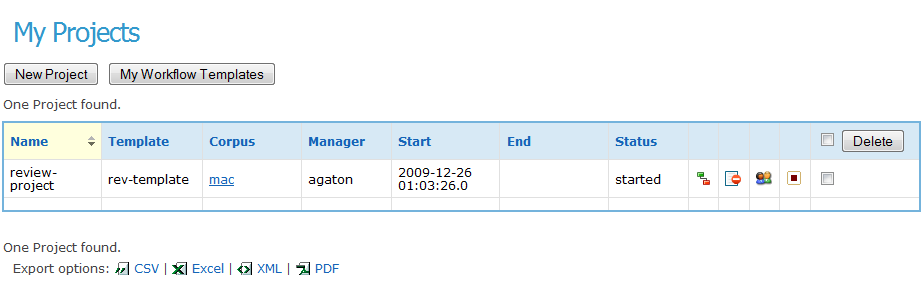
\includegraphics[scale=0.4]{myprojects}
\caption{My Projects}
\label{fig:myprojects}
\end{figure}
For each project, there are several available options (four icons next to the
Status field as shown in Figure~\ref{fig:myprojects}):
\begin{itemize}
  \item \texttt{view processes} for the particular project,
  \item \texttt{suspend/resume} the project,
  \item \texttt{change the project actors}: managers, curators, annotators,
  \item \texttt{end} the project,
  \item \texttt{delete} the project.
\end{itemize}
Besides that, after project is completed, you will be notified by email.
All these options are described in detail in the following subsections.

\subsection{Project Processes}
In order to see project processes, click on \emph{Processes} icon (red and 
green icon, see Figure~\ref{fig:myprojects}) for the specific project listed in
the \emph{My Projects} page.
The process list will be shown as in Figure~\ref{fig:processesinproject}:
\begin{figure}[htb]
\centering
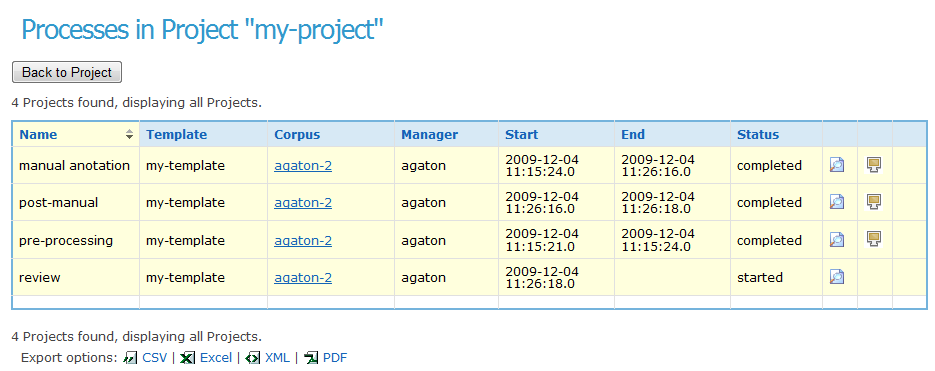
\includegraphics[scale=0.4]{processesinproject}
\caption{Project Processes}
\label{fig:processesinproject}
\end{figure}:
From the \emph{Processes} page, you can:
\begin{itemize}
  \item \texttt{see the status} of each process (started, suspended or
completed),
  \item \texttt{monitor processes} by clicking on \emph{Process Monitoring}
icon. For
details on process monitoring console see details in Section
~\ref{section:process-monitoring}.
  \item \texttt{view tasks} created for each process by clicking on \emph{View
Tasks} icon (see Figure~\ref{fig:taskinstances}).
\begin{figure}[htb]
\centering
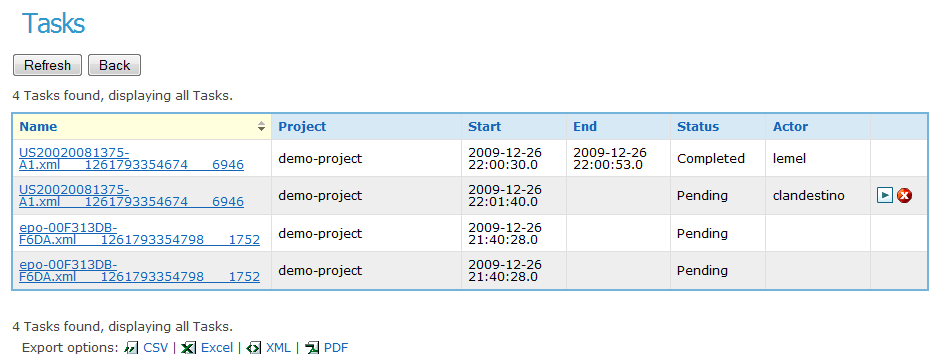
\includegraphics[scale=0.4]{taskinstances}
\caption{Task List}
\label{fig:taskinstances}
\end{figure}
When annotators start to annotate, you will be able to see the list of tasks and
their status. For example, if there are 2
documents in the corpus and 2 annotators are assigned to annotate each document,
there will be 4 tasks in total as shown in Figure~\ref{fig:taskinstances}.
In this example, one annotator finished task, the other annotator accepted the task,
and two left tasks have not been taken yet.
From the Task List page you can also see who is the assigned user, and start and
end times for specific tasks.
Should you want to finish or cancel annotator task, you can do that by
clicking on relevant icons. These actions correspond to \emph{canceling
document annotation} and \emph{returning document to the pool} respectively.
\end{itemize}

\subsection{Suspend/Resume Project}
 A project can be suspended at any time, by clicking on \emph{Suspend} icon.
This means that all processes and tasks in that project will be suspended.
The project can be resumed later, which analogly will result in resuming
its processes and tasks.
This is shown in Figure~\ref{fig:suspendproject}:
\begin{figure}[htb]
\centering
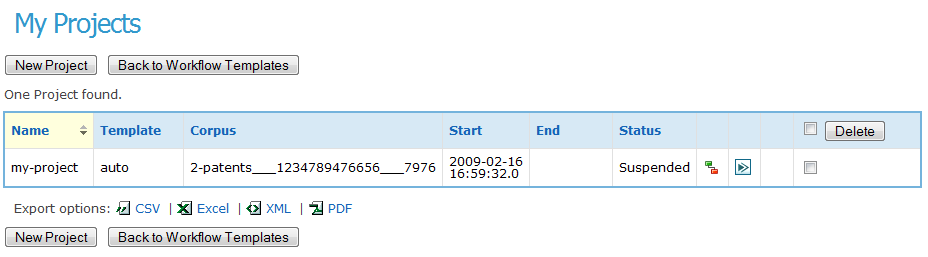
\includegraphics[scale=0.4]{suspendproject}
\caption{Suspend Project}
\label{fig:suspendproject}
\end{figure}

\subsection{Change Project Actors}
There is often a need to change actors during project execution.
For example, you might want to pass manager role to someone else or to change
curators and annotators due to some changes in personnel. This option is
available in GATE Teamware.
From the \emph{My Projects} page you need to click on \emph{Change Actors} icon
for the specific project, and you will be redirected to the page where you can
change all actors as shown in Figure~\ref{fig:changeprojectactors}.
\begin{figure}[htb]
\centering
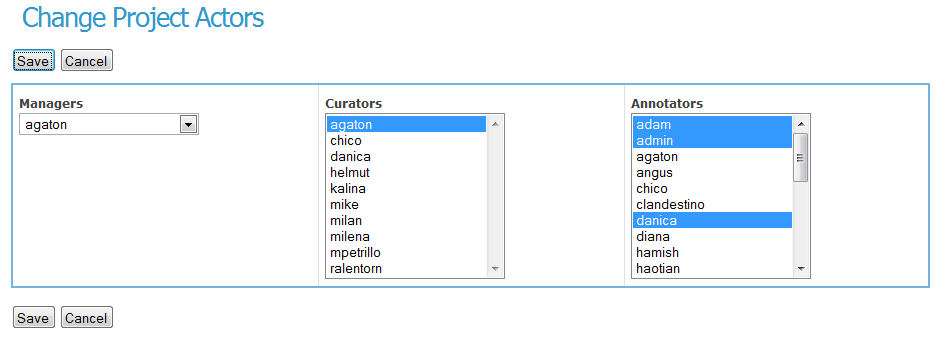
\includegraphics[scale=0.4]{changeprojectactors}
\caption{Change Project Actors}
\label{fig:changeprojectactors}
\end{figure}
As it is visible in Figure~\ref{fig:changeprojectactors}, the current
actors will be preselected.

\subsection{End Project}
 A project can be ended at any time, by clicking on \emph{End} icon (the first
 on the right). This means that all processes and tasks in that project will be
 ended. The project cannot be resumed later. This option is useful if manager wants to 
stop the work on the project, but leave the project history intact.
This is shown in Figure~\ref{fig:endproject}:
\begin{figure}[htb]
\centering
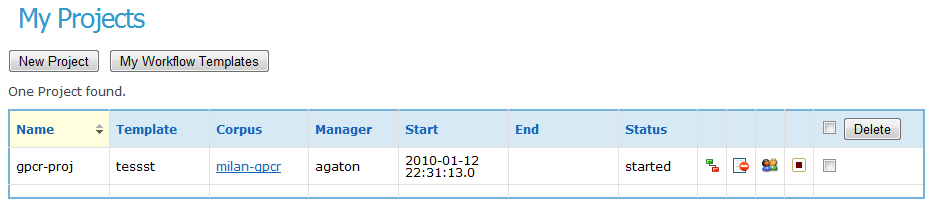
\includegraphics[scale=0.4]{endproject}
\caption{End Project}
\label{fig:endproject}
\end{figure}

\subsection{Delete Project}
With time, the number of your projects will increase, therefore we provide the
option to delete old projects.
It is not restricted only to completed projects, so you can delete even 
running projects. Deleting a project will also delete the
corresponding processes and tasks.

\subsection{Email Notification}
As a manager you will be notified by email, upon your project completion.
This can be very useful, if you are not actively monitoring execution.
The example of email you can expect is shown on
Figure~\ref{fig:projectcompletednotification}.
\begin{figure}[htb]
\centering
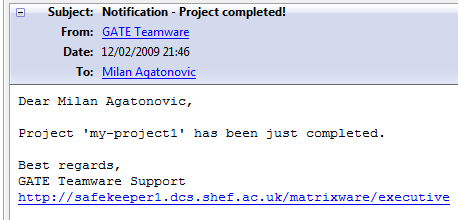
\includegraphics[scale=0.4]{projectcompletednotification}
\caption{Project Completed Notification}
\label{fig:projectcompletednotification}
\end{figure}
\section{Process Monitoring}\label{section:process-monitoring}

Here we will introduce Process monitoring console for real-time
monitoring and gathering information about currently executing processes.
The main idea behind this functionality is to:
\begin{itemize}
  \item isolate annotation process failures,
  \item improve annotation process performance,
  \item help making decisions, and
  \item improve resource management.
\end{itemize}

At the moment, GATE Teamware provides four different views in process
monitoring console:
\begin{itemize}
  \item Document Status Summary
  \item Annotation Status Details
  \item Annotator Record Summary
  \item Record Summary for All Annotators
\end{itemize}

Each view is explained in details in the following subsections.

\subsection{Document Status Summary}
To access this page, click on \emph{Process monitoring} icon in the
process list for particular project. You will see the progress of the
annotation process both in tabular and graphical
view using pie chart as shown in Figure~\ref{fig:annotationstatusoverview}.
\begin{figure}[htb]
\centering
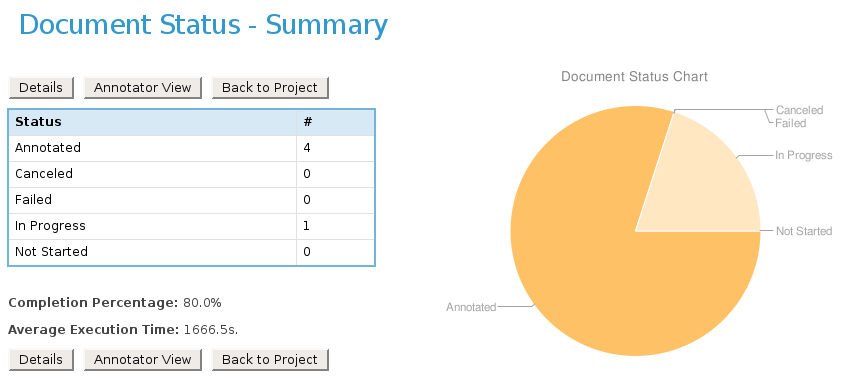
\includegraphics[scale=0.4]{annotationstatusoverview}
\caption{Document Status Summary}
\label{fig:annotationstatusoverview}
\end{figure}
The progress is displayed in real time so that it is possible
 to monitor how many documents have been finished, canceled, annotated, failed,
 in progress, and not started. When the annotation process ends, the pie chart
will disappear.

\subsection{Document Status Details}
Annotation Status Overview gives pretty condensed view about what is going on
inside process.
For more detailed view, click \emph{Details} button, and you will see the
details of the annotation project progress by document, including names of
annotators who started the work on it, finished or
 rejected the document as shown in Figure~\ref{fig:annotationstatusdetailedview}
\begin{figure}[htb]
\centering
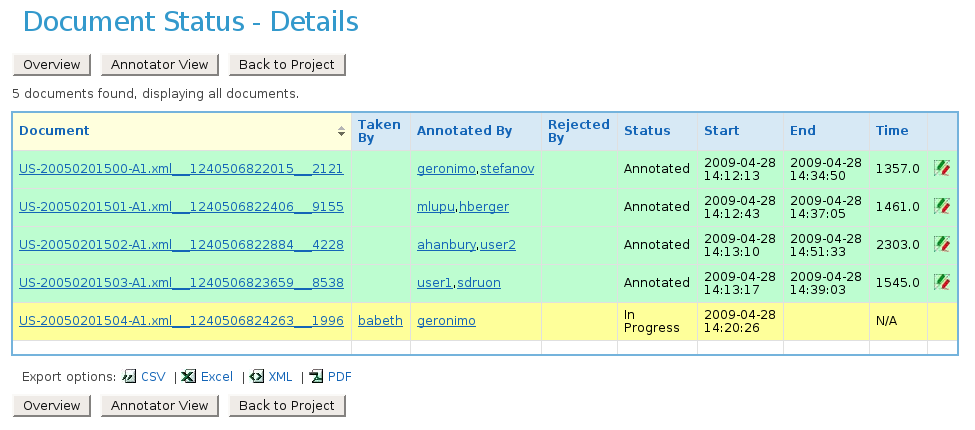
\includegraphics[scale=0.4]{annotationstatusdetailedview}
\caption{Document Status Details}
\label{fig:annotationstatusdetailedview}
\end{figure} 
 
 From this list, the status of the documents is also
 visible together with the execution time per document. For specific documents in
 the list it is possible to view details such as:
 \begin{itemize}
   \item \texttt{view (annotated) documents}, by following the document
name link. This will launch \emph{Annotation Editor}, which is described in
Section ~\ref{section:annotation-editor}
   \item \texttt{compare document annotations}; to do this follow the icon
at the end of the \emph{annotated} document row. The document with
   annotations will be loaded into the \emph{Annotation Differ} application,
which is described in Section ~\ref{section:annotation-differ}
\end{itemize}
 
\subsection{Annotator Record View}
Both annotation status views explained above are focused on the document
itself, while there might be the cases when the manager wants to see how
particular annotator performed. Therefore, we have implemented \emph{Annotator
Record View}, which you can access by clicking on the annotator name from
\emph{Document Status Details} page.
You will be able to see how many documents annotator completed, canceled,
started to annotate, along with some useful metrics. A sample \emph{Annotator
Record View} page is shown in Figure~\ref{fig:annotatorrecordview}:
\begin{figure}[ht!]
\centering
\includegraphics[scale=0.4]{annotatorrecordview}
\caption{Annotator Record View}
\label{fig:annotatorrecordview}
\end{figure}


\subsection{Record Summary for All Annotators}
In case that manager is interested to see how workload is shared among
annotators with an indicator about the average time spent per document,
\emph{Record Summary for All Annotators} screen can be very useful.
You can see this screen by clicking on \emph{Annotator View} button.
An example of this screen is shown in
Figure~\ref{fig:globalannotatorrecordview}: 
\begin{figure}[ht!]
\centering
\includegraphics[scale=0.4]{globalannotatorrecordview}
\caption{Global Annotator Record View}
\label{fig:globalannotatorrecordview}
\end{figure}




\chapter{Support}
This chapter details Support module which includes: forum, chat and tutorials.
\section{Forum}
GATE Teamware includes forum powered by \url{http://www.jforum.net}.
The complete list of features is available at:
\url{http://www.jforum.net/features.jsp}.

The forum is envisaged to serve as the primary way for interactive support, instead of mailing list.
As with any advanced forum, users can post new messages and replies, or create new topics. 

Figure~\ref{fig:forum} depicts the main forum page with list of available forums. 

Feel free to use this forum to post any particular questions, report bugs and suggest any new features for the GATE Teamware.
\begin{figure}[hb!]
\centering
\includegraphics[scale=0.4]{forum}
\caption{Forum home page}
\label{fig:forum}
\end{figure}

Users with \emph{administrator} role can change forum settings and create new forums and categories. This is accomplished through the adiministration panel shown in Figure~\ref{fig:forumadmin} below.

\begin{figure}
\centering
\includegraphics[scale=0.4]{forumadmin}
\label{fig:forumadmin}
\end{figure}

\section{Chat}

Chat is still in experimental phase. Currently, this service is very basic, as shown in Figure~\ref{fig:chat}).
\begin{figure}[hb!]
\centering
\includegraphics[scale=0.4]{chat}
\caption{Chat Window}
\label{fig:chat}
\end{figure}

Message is broadcasted to all logged users. This is implemented with the idea to see if such functionality can be of interest to the users.
\section{Help}
Apart from this user guide, in this section you will find several movie tutorials which can help you to familiarise yourself with the GATE Teamware interface and functionalities.
% \begin{figure}[hb!]
% \centering
% \includegraphics[scale=0.4]{help}
% \caption{Help Window}
% \label{fig:help}
% \end{figure}


\end{document}